\chapter{Análise dos Controles}
\label{c.analise}

A fim de avaliar tecnologias sob o aspecto de uso, \citeonline{mcnamara} propuseram uma estrutura que se baseia em três aspectos: funcionalidade, experiência e usabilidade. A funcionalidade leva em consideração as características técnicas do dispositivo, experiência foca no relacionamento entre o usuário e a tecnologia e a usabilidade nas características de interação entre o usuário e o dispositivo. Os dispositivos utilizados para a realização da análise podem ser visualizados na Figura ~\ref{f.controles}. O controle via cabo utilizado acompanha o console de vídeo game \textit{Playstation 2} e é referenciado neste trabalho como PS2. 

\begin{figure}[H]
	\caption{\small Controles utilizados na análise}
	\centering
	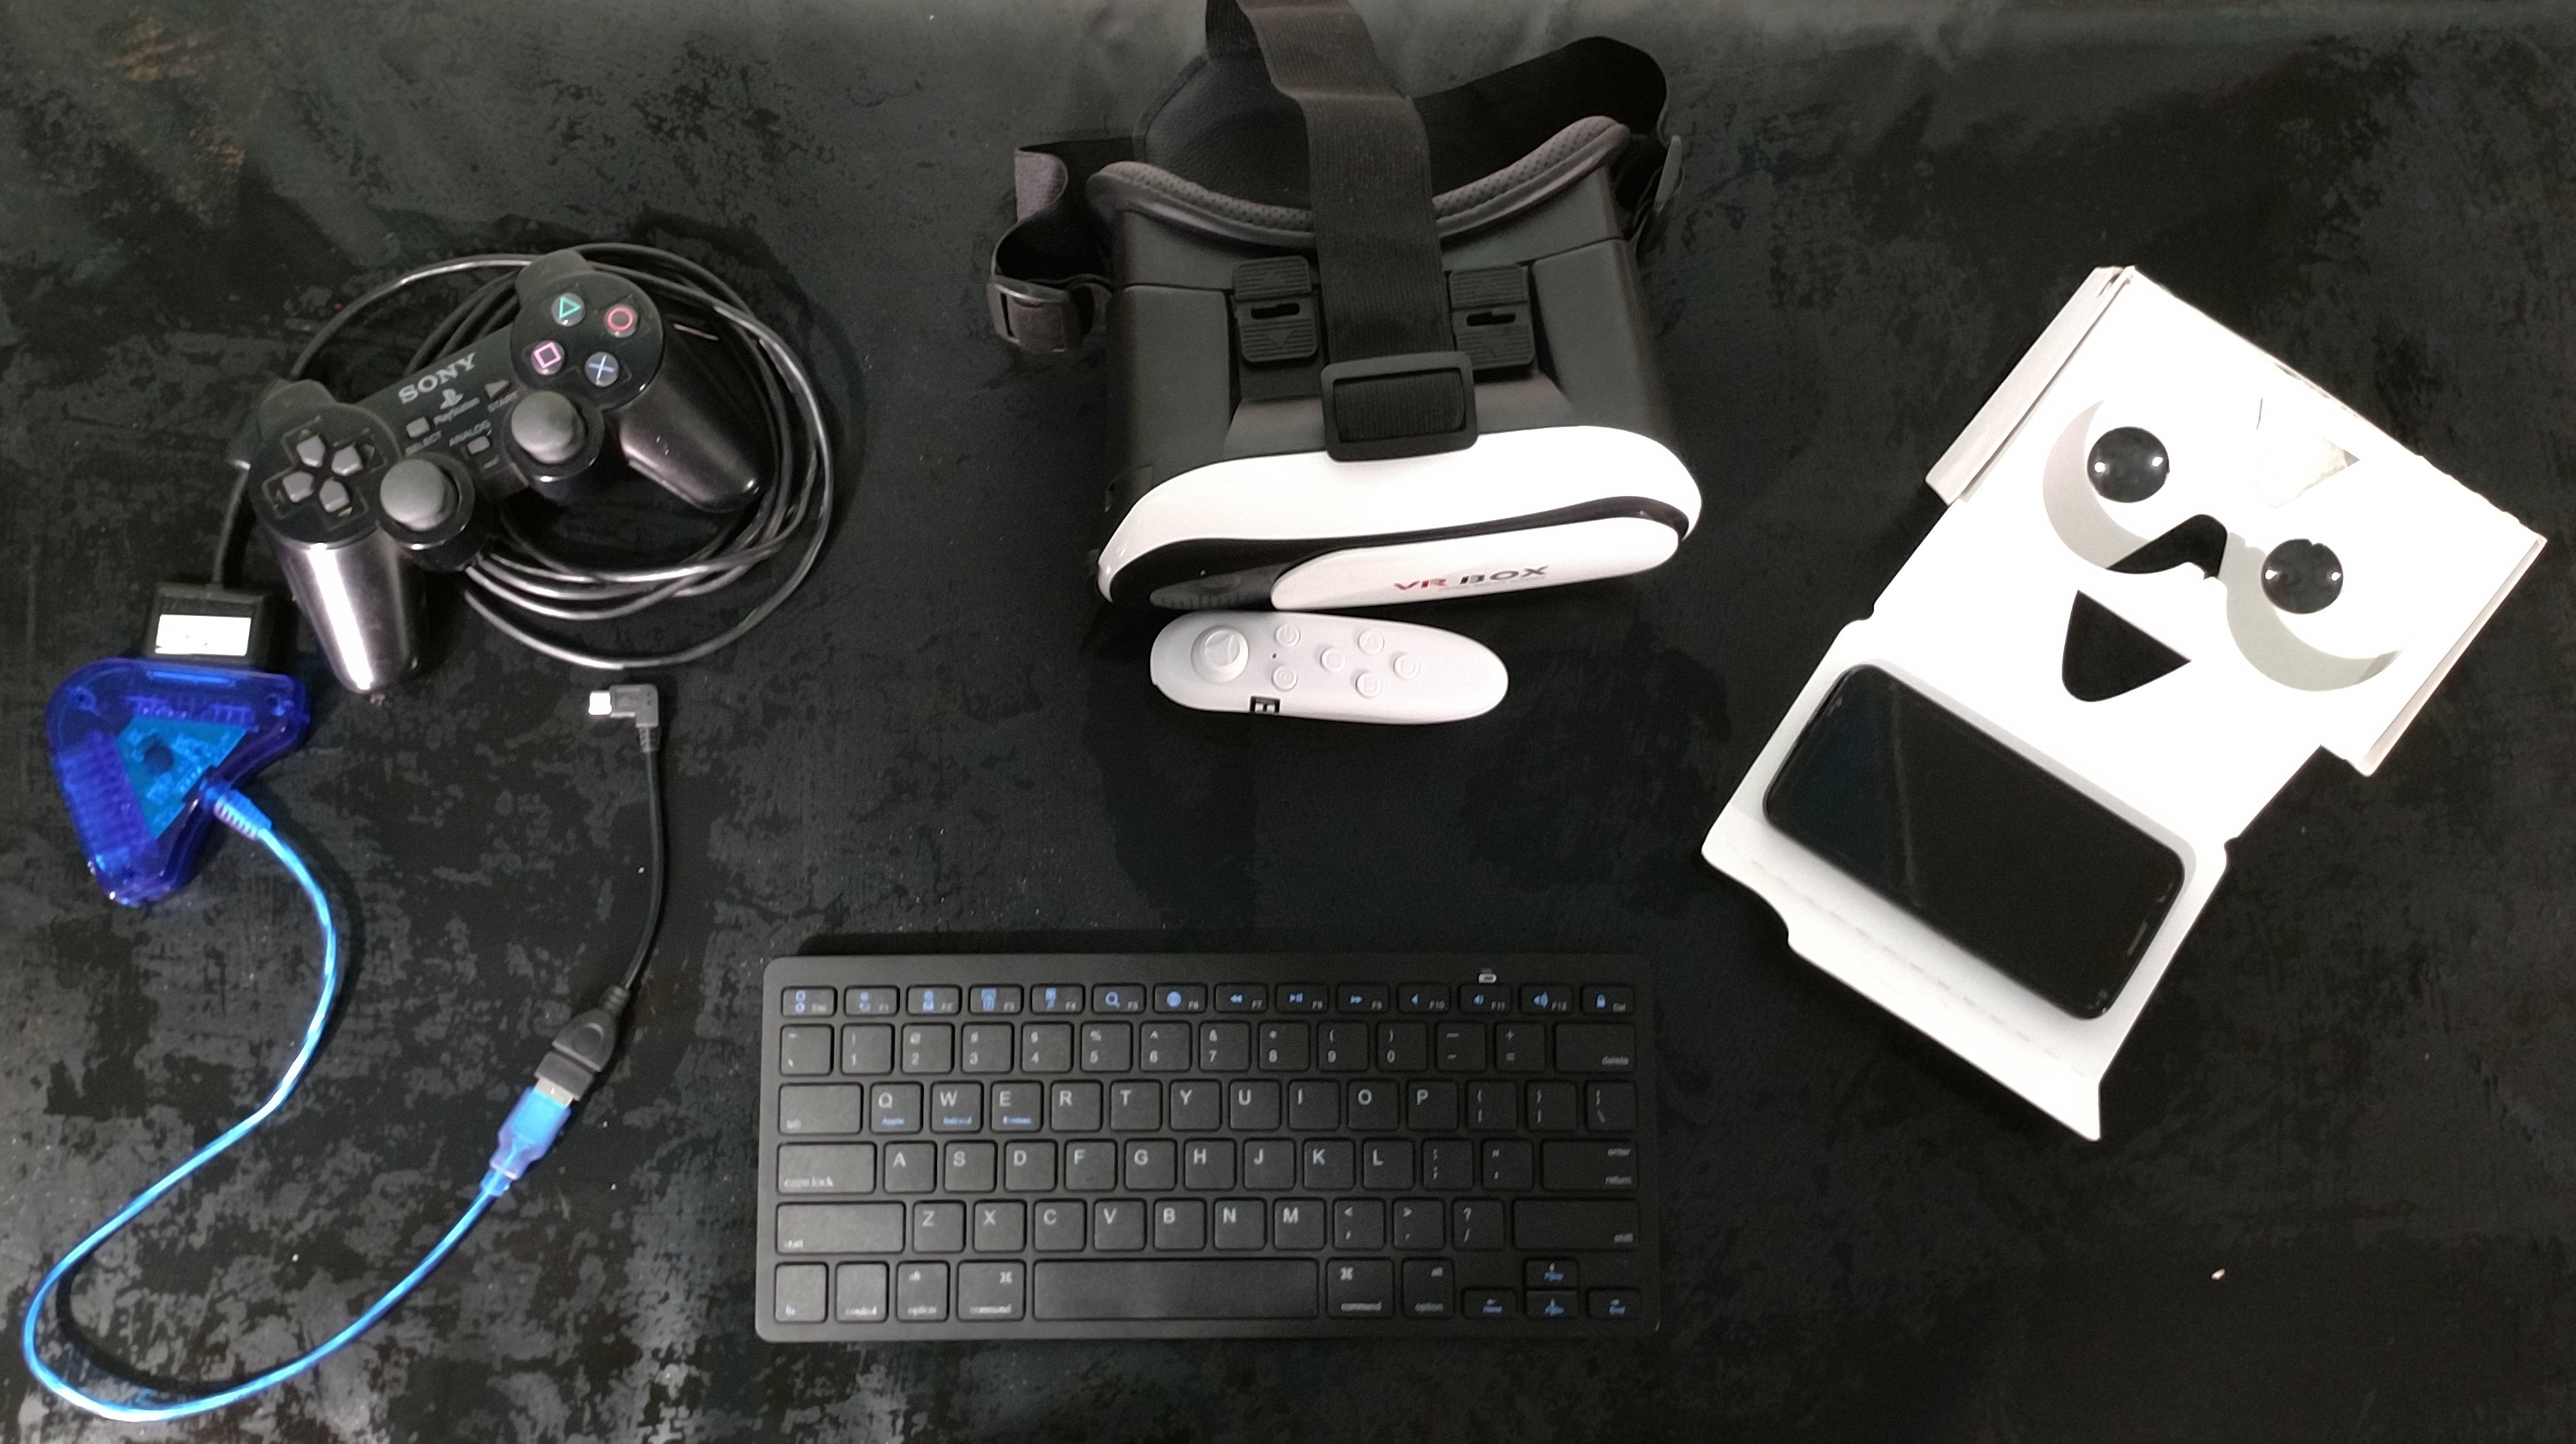
\includegraphics[height=7cm]{Imagens/controles.jpg}
	\label{f.controles}
	\legend{\small Fonte: Elaborada pelo autor.}
\end{figure}

\section{Funcionalidade}
\label{funcionalidade}

Segundo \citeonline{mcnamara}, para avaliar a funcionalidade de um dispositivo pode-se analisar a performance, confiabilidade e durabilidade do mesmo. A quantidade de funções que um dispositivo oferece também deve ser considerada pois muitas opções de entrada podem inutilizar muitos comandos e poucas podem ser insuficientes. \citeonline{brown} afirma que a funcionalidade é um aspecto de interação que é relativamente independente do ambiente e do usuário. 

Quanto à performance, a característica analisada foi se o dispositivo ofereceu resposta rápida aos comandos do usuário, ou seja, se foram observados atrasos na comunicação entre o dispositivo e o celular. A facilidade de conexão do controle ao dispositivo móvel e a preservação desta conexão são características de confiabilidade. Por fim, a durabilidade levou em consideração o tipo de material de cada controle e se houve ou não falhas mecânicas na execução de comandos.

A análise foi feita com base em observações feitas pela autora onde cada controle foi utilizado para interagir com a aplicação desenvolvida. Cada controle foi analisado por em média dois minutos (tempo médio para destruir todos os focos de dengue apresentados na aplicação).

O Google Cardboard 2.0 mostrou ser o controle mais fácil de ser utilizado. Por não necessitar de conexão com o celular, a aplicação pôde ser inicializada rapidamente e não houve problemas técnicos durante a execução. Como o sistema de interação é o toque na tela, não foram observados nenhum atraso de resposta ou falhas mecânicas ao pressionar o botão. Em relação ao material, o Google Cardboard 2.0 é o que apresenta maior fragilidade em relação aos demais. Por ser quase inteiramente feito de papelão, o visualizador tem grandes chances de apresentar problemas em sua estrutura em um curto período de tempo. 

O segundo controle avaliado foi o PS2. Este possui uma qualidade de material superior em relação ao primeiro, porém, a conexão com o dispositivo não se manteve estável durante os testes. Isto ocorreu devido à problemas de compatibilidade com o Android 5.1 (\textit{Lollipop}), que não reconhece certos dispositivos através do cabo OTG. Testes realizados com um dispositivo Android 6.0 (\textit{Marshmallow}) não apresentou problemas de conexão. Para que o sistema utilizasse o controle como dispositivo de entrada, foi necessário instalar um aplicativo que funcionou como \textit{driver} para o controle utilizado, o que também dificultou a conexão inicial do dispositivo. O controle PS2 também não apresentou atrasos de resposta ou falhas mecânicas durante a análise.

Os controles \textit{Bluetooth} (\textit{joystick} do VR Box e teclado) apresentaram dificuldade na conexão inicial pois, diferentemente do cabo OTG, foi necessário conectar os dispositivos manualmente. Contudo, estes controles não apresentaram atrasos de resposta ou problemas de conexão. Além disso, a qualidade do material também mostrou ser superior ao Google Cardboard 2.0.

\section{Usabilidade}

A usabilidade, segundo a ISO 9241-11 \cite{iso9241} tem como objetivo definir usabilidade e explica como identificar a informação necessária para avaliação de usabilidade de um computador em termos de medidas de desempenho e satisfação do usuário, ou seja, mede o quanto um usuário específico pode utilizar um produto e atingir os seus objetivos com eficácia, eficiência e satisfação em um contexto específico de uso.

De acordo com \citeonline{brown}, eficácia descreve a habilidade do usuário em realizar uma tarefa com a tecnologia. Eficiência considera os recursos utilizados para realizar a tarefa, podem ser esforço mental, esforço físico ou tempo. A satisfação mede o quanto a interação impactou o usuário, devendo ser extraída somente através de respostas do usuário. 

Os questionários aplicados neste estudo tiveram como base a ISO 9241-9 e o trabalho de \citeonline{lewis} que é citado na ISO 9241-11 e oferece modelos de questionários para avaliação da satisfação de um produto. Por fim, o contexto de uso leva em consideração não somente o ambiente físico mas também as características individuais dos usuários. 

Para acessar a usabilidade oferecida por cada controle, 7 voluntários utilizaram a aplicação com os quatros diferentes controles e responderam a dois questionários elaborados por \citeonline{lewis}. O primeiro questionário é denominado \textit{"The After-Scenario Questionnaire (ASQ)"} (Apêndice ~\ref{a.apendice1}) e foi respondido para quatro cenários: andar, eliminar um foco de dengue, agachar e retornar ao menu. Este questionário possui apenas três questões que medem a facilidade para completar uma tarefa, tempo para completar a tarefa e se o suporte foi adequado. Como a análise é restrita aos controles e não à aplicação em si, o ASQ utilizado contém somente duas questões, já que problemas com o suporte não foram considerados. O segundo questionário, denominado \textit{"The Post-Study System Usability Questionnaire (PSSUQ)"} (Apêndice ~\ref{a.apendice2}) foi utilizado após a experiência completa da aplicação e foi respondido para cada controle. Como no primeiro questionário, questões que levavam em consideração a aplicação foram removidas. Ambos os questionários utilizam uma escala de 1 a 7 para cada pergunta sendo que 1 corresponde à "concorda totalmente" e 7 "discorda totalmente". No final, é feito a média aritmética das notas onde menores médias representam melhores avaliações.  

No total, 3 homens e 4 mulheres participaram da análise. A média de idade foi de 22,14, com idades variando entre 20 e 23 anos. Também foi questionado se os participantes possuíam experiência com algum dos controles apresentados e se já haviam utilizado aplicações em RV. Todos os participantes responderam que possuíam experiência com o teclado e o PS2, dois dos participantes disseram que também possuíam experiência com o Google Cardboard e apenas um deles já teve contato com todos os controles apresentados. Todos os voluntários já haviam entrado em contato com aplicações em RV.

Os resultados do ASQ podem ser visualizados na Tabela ~\ref{t.ASQ}.

\begin{table}[H]	
	\caption{Resultados após cada cenário (ASQ)} 
	\label{t.ASQ} 
	\centering
	\begin{tabular}{l|l}
	\textbf{\small Dispositivos } & \textbf{\small Média Aritmética} \\\hline
	
	{\small Google Cardboard 2.0} & {\small 1,75}  \\\hline	
	
	{\small Controle PS2} & {\small 1,43}  \\\hline		 
	
	{\small Controle VR Box} & {\small 1,43}  \\\hline  
	
	{\small Teclado} & {\small 1,79} \\\hline	
	\end{tabular}
	\legend{\small Fonte: Elaborada pelo autor}	
\end{table}

Os resultados apresentados mostraram que os controles PS2 e VR Box (\textit{joystick} que acompanha o visualizador) tiveram o melhor desempenho nos cenários propostos, apresentando maior facilidade e rapidez no uso de acordo com os participantes. A fim de saber se houve diferença significativa entre os resultados obtidos para cada controle, foi realizado a análise de variância ANOVA. O procedimento verifica se as médias de dois ou mais grupos são iguais através da comparação das variâncias dentro de cada grupo e entre os grupos \cite{minitab}. Esta comparação resulta no valor F que, se for menor do que o valor de F crítico (calculado pelo \textit{software} utilizado), então é possível concluir que não existe diferença entre as médias no ponto de vista estatístico. Este resultado é comprovado se o valor p é maior do que alfa (o valor padrão utilizado para alfa é 0.05). Neste experimento, cada grupo foi representado por um controle distinto.

Ao realizar a análise de variância ANOVA (Figura ~\ref{f.anovaasq}) por meio do \textit{software} Excel, foi constatado que não existe variância significativa entre os controles testados (F < F-crit). Porém, é importante observar que, ao aumentar a quantidade de cenários apresentados, alguns controles podem não apresentar suporte para ações extras. É o caso do Google Cardboard 2.0 que, por apresentar somente um botão, possui limitação para o número de ações. Já o teclado, por apresentar muitas opções de entrada, acaba tendo muito da sua capacidade inutilizada. 

\begin{figure}[H]
	\caption{\small Análise ANOVA para o ASQ.}
	\centering
	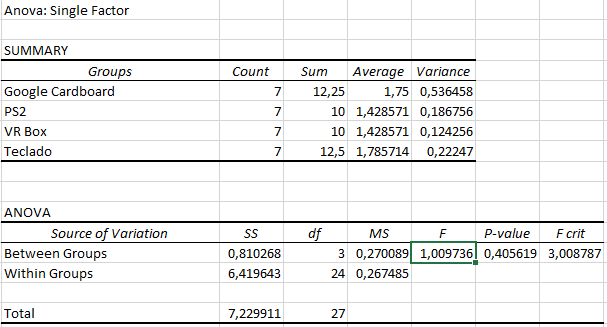
\includegraphics[scale=0.7]{Imagens/anovaasq.png}
	\label{f.anovaasq}
	\legend{\small Fonte: Elaborada pelo autor.}
\end{figure}

As avaliações de cada controle seguindo o questionário PSSUQ pode ser visualizado na Tabela ~\ref{t.PSSUQ}. 

\begin{table}[H]	
	\caption{Resultados após cada controle (PSSUQ)} 
	\label{t.PSSUQ} 
	\centering
	\begin{tabular}{l|l}
		\textbf{\small Dispositivos } & \textbf{\small Média Aritmética}\\\hline
		
		{\small Google Cardboard 2.0} & {\small 1,68} \\\hline	
		
		{\small Controle PS2} & {\small 1,33} \\\hline		 
		
		{\small Controle VR Box} & {\small 1,47	}  \\\hline  
		
		{\small Teclado} & {\small 2,04	 } \\\hline	
	\end{tabular}
	\legend{\small Fonte: Elaborada pelo autor}	
\end{table}

Os controles melhores avaliados pelos participantes, como no primeiro questionário, foram os controles PS2 e VR Box. A análise ANOVA (Figura ~\ref{f.anovapssuq}) demonstrou que não existe diferença significativa entre os controles (F < F-crit), porém, a variância de notas entre os controles foi maior no questionário PSSUQ. Apesar de todos os participantes terem experiência com os controles PS2 e teclado, é evidente a preferência ao PS2 para interagir com a aplicação. Observações realizadas durante o experimento constataram que os participantes tiveram dificuldade para segurar o teclado de forma confortável, o que poderia justificar a sua baixa avaliação. 

\begin{figure}[H]
	\caption{\small Análise ANOVA para o PSSUQ.}
	\centering
	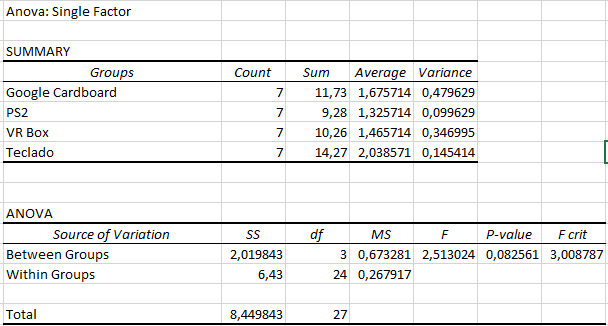
\includegraphics[scale=0.7]{Imagens/anovapssuq.png}
	\label{f.anovapssuq}
	\legend{\small Fonte: Elaborada pelo autor.}
\end{figure}

\section{Experiência}
\label{experiencia}

De acordo com \citeonline[tradução nossa]{benyon}, a experiência “remete à todas as qualidades do sistema interativo que o fazem memorável, satisfatório e gratificante.” Tendo em mente os controles de interação, usuários podem obter uma experiência negativa se as características de funcionalidade forem insatisfatórias e se houver problemas para encontrar os botões corretos no controle, já que neste caso poderá ser necessária a remoção do capacete de visualização resultando em uma interrupção da experiência em RV. 

Para verificar a experiência oferecida por cada controle, foi perguntado aos usuários qual dos quatro controles resultou em uma melhor experiência. Adicionalmente, eventuais comentários feitos pelos participantes sobre os controles foram anotados e separados entre positivos e negativos. 

O resultado do experimento mostrou que os controles PS2 e VR Box foram os controles preferidos dos participantes com 3 votos cada, o voto remanescente foi para o Google Cardboard 2.0. O controle que menos agradou os participantes foi o teclado, que obteve 4 votos, seguido do Google Cardboard 2.0 que totalizou 3 votos.

Ao observar os participantes, foi possível notar que o cabo do PS2 era muito longo e houve uma preocupação por parte dos usuários para remover o cabo do caminho. No entanto, este detalhe não interferiu de forma significativa na preferência dos usuários pelo controle pois, segundo cometários dos participantes, o PS2 propiciou conforto durante os testes e, como todos os participantes declararam ter experiência utilizando o controle, nenhum apresentou dúvidas quanto ao posicionamento dos botões.

Quanto ao controle \textit{Bluetooth} VR Box, foram constatados opiniões diversas, todas em relação ao seu tamanho. Alguns participantes declararam que os botões ficavam muito juntos o que dificultava a interação, outros comentaram que o controle se encaixa na mão com facilidade.

O teclado foi o controle que recebeu mais opiniões negativas o que pode ser justificado pelo tamanho do dispositivo e pela quantidade de funções que ele oferece. Durante o experimento, os usuários mostraram ter dúvidas sobre qual seria a melhor maneira de segurar o teclado, algo que não ocorreu com os outros controles. Além disso, o número de entradas de dados disponível no controle é muito maior do que o exigido pela aplicação, o que deixou muitas teclas sem utilidade e aumentou as chances de erro do usuário ao utilizar a aplicação. 

Por fim, o Google Cardboard 2.0 recebeu elogios quanto à sua facilidade de uso. Porém, alguns usuários se queixaram que era preciso segurar o controle durante a experiência. Além disso, para retornar ao menu principal (um dos cenários apresentados) era necessário selecionar um botão localizado no ambiente e, para isso, o usuário precisou caminhar até o local ao invés de simplesmente acionar outro botão, resultando em um maior esforço em comparação com os outros controles.  
  
